\chapter{Linked List Implementation} % Write in your own chapter title
\label{Chapter5}
\lhead{Chapter 5. \emph{Linked List Implementation}}
\section{Methodology}
Singley linked lists are used to carryout basic operations on the data array. These basic operations and their working are as follows:

\subsection{Insertion}
Insertion is done by dynamically allocating nodes. Keys i.e., ID's of employees and data is linked with these node. Finally, nodes are inserted at the head of the list.

Time Complexity: \textbf{O(1)} \\
Space Complexity: \textbf{O(N)}

\subsection{Finding}
There is no order in the linked list data like trees so find operation is carried out by simply traversing the list until the required key is found or tail of the list is reached.

Time Complexity: \textbf{O(N)} \\
Space Complexity: \textbf{O(N)}

\subsection{Sorted Traversal}
For sorted traversal, first of all list should be sorted by any convenient sorting algorithm and then traversed from head to tail.

Sorting Algrithm Used: \textbf{Quick Sort O(log N)} \\
Time Complexity: \textbf{O(N log N)}\\ 
Space Complexity: \textbf{O(N)} \\
\textit{Note: Sorted traversal time complexity is dependent upon sorting algorithm used.}\\
\subsection{Deletion}
Deletion is carried out by finding the node to be deleted. This step involves traversing the list. After finding, the node is bypassed by link adjusment and is deleted. 

Time Complexity: \textbf{O(N)} \\
Space Complexity: \textbf{O(N)}

	
\section{Execution Times and Memory Consumptions}
\begin{figure}[H]
	\centering
	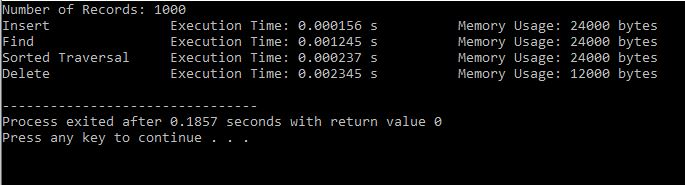
\includegraphics[scale =0.7]{./Figures/List1000.jpg}
	\rule{35em}{0.5pt}
	\caption{Results for linked list implementation with data size 1000.}
	\label{fig:List 1000}
\end{figure}

\begin{figure}[H]
	\centering
	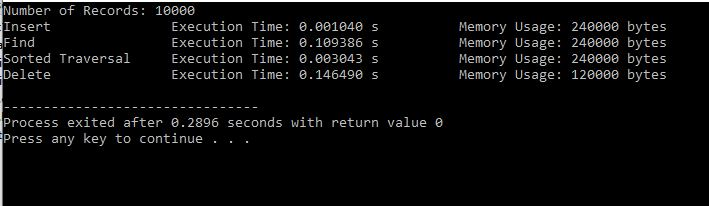
\includegraphics[scale =0.7]{./Figures/List10000.jpg}
	\rule{35em}{0.5pt}
	\caption{Results for linked list implementation with data size 10000.}
	\label{fig:List 10000}
\end{figure}

\begin{figure}[H]
	\centering
	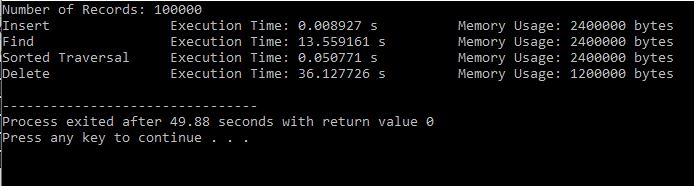
\includegraphics[scale =0.7]{./Figures/List100000.jpg}
	\rule{35em}{0.5pt}
	\caption{Results for linked list implementation with data size 100000.}
	\label{fig:List 100000}
\end{figure}